\documentclass[UTF8]{ctexart}
%\usepackage[margin=1.5cm]{geometry} %設定四個邊界皆為 1.5 cm
\usepackage[left=2cm, right=2cm, top=1.5cm, bottom=1.2cm]{geometry} %設定左邊界2cm,右邊界2cm,上邊界1.5cm, 下邊界 1.2cm
\setlength{\parindent}{0pt} %開頭不縮排

\usepackage{mathtools}

\usepackage{pgfplots}       % 使用pgfplots繪圖工具包
\pgfplotsset{width=7cm,compat=1.13} % 圖片繪制的寬度是7cm,使用的pgfplots版本是1.13

\usepackage{graphicx} %插入圖片函式庫
\usepackage{caption}
\usepackage{subfigure}

\begin{document}
\begin{CJK*}{UTF8}{song}
%\thispagestyle{empty} %首頁頁碼空白
\setlength{\baselineskip}{20pt} %全部行距皆為 30 points

%標題
\begin{center}
\begin{LARGE} 
\textbf{Quantum Analogs Experiment 結報} \\
\end{LARGE}
\begin{large} 
B5組 0412107 陳麒升、0412001 陳勁宇  
\end{large}
\end{center}

%%%%%%%%%%%%%%%<1頁%%%%%%%%%%%%%%%%%%
%動機
\begin{large}
\textbf{1.實驗動機與目的:} \\
\end{large}
分別利用手動與音效卡操作聲波實驗裝置以模擬氫原子波函數,觀察裝置resonance frequencies之相關性質。 \\
 \\
%
% 你認為或發現的實驗操作重點方式,條列式 ≤ 五項
\begin{large}
\textbf{2.實驗操作重點方式:} \\
\end{large}
◆於手動實驗操作方面我們組別認為需要注意的有: \\
(1) 注意線路品質、線路是否都能穩定收發訊號。 \\
(2) 注意一定要登記attenuator之刻度值,並於實驗中該值需要維持固定。 \\
(3) 於尋找震幅極值時調整頻率盡量精確到個位數。 \\
◆於音效卡自動掃頻實驗操作方面我們組別認為需要注意的有: \\
(1) 將Atom Analog金屬雙半球裝置於實驗時盡可能遠離電腦主機(例如我們進行實驗時將莊置平穩放於椅子上操作),可以有效避免主機運作時震動所帶來的掃頻誤差。 \\
(2) 於最後繪製 $Y^{0}_{x}(\theta,\varphi)$ 之極座標作圖時掃描時間不可太大(本實驗我們組改動預設的10秒為0.1秒)。  \\
%
%%%%%%%%%%%%%%%%%%%%%%%%%%%%%%%%%%%%%%


%%%%%%%%%%%%%%%2~5頁%%%%%%%%%%%%%%%%%%
% 附課堂上操作的原始數據資料等
\begin{large}
\textbf{3.實驗raw data:} \\
\end{large} 
(1)實驗裝置振幅($mV$)-頻率($Hz$) 關係圖 :\\ 
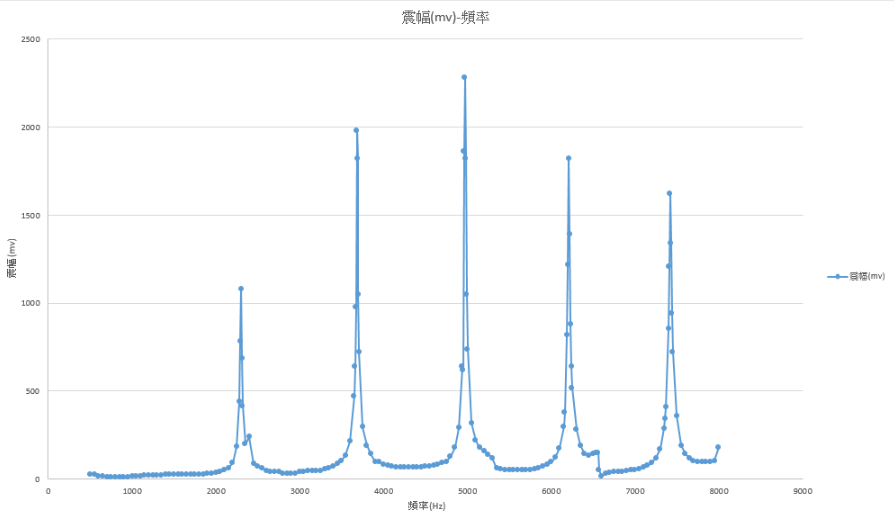
\includegraphics[width = .9\textwidth]{exp1.png}  \\  %匯入同路徑下圖片 這樣圖片的寬度會被縮放至頁面寬度的百分之八十,圖片的總高度會按比例縮放。
 \\
\newpage %強制分頁

(2)各頻率($Hz$)之振幅($mV$)-弧度($rad$) 關係圖: \\
◆$2300 Hz$ \\
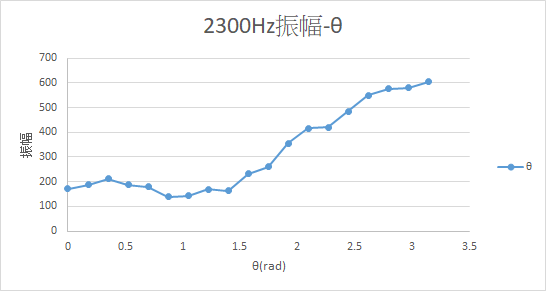
\includegraphics[width = .6\textwidth]{2300hz.png} \\
◆$3690 Hz$ \\
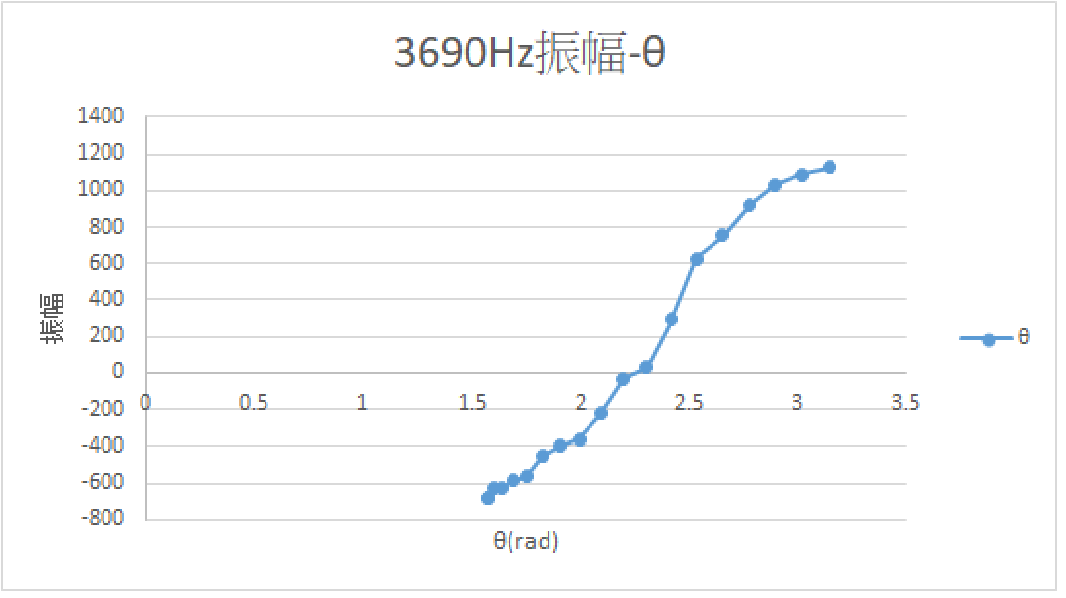
\includegraphics[width = .6\textwidth]{3690hz.png} \\
◆$4975 Hz$ \\
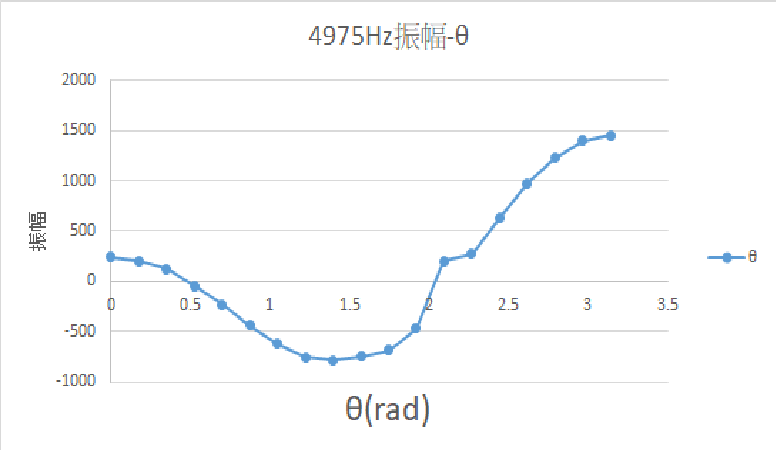
\includegraphics[width = .6\textwidth]{4975hz.png} \\
◆$6218 Hz$ \\
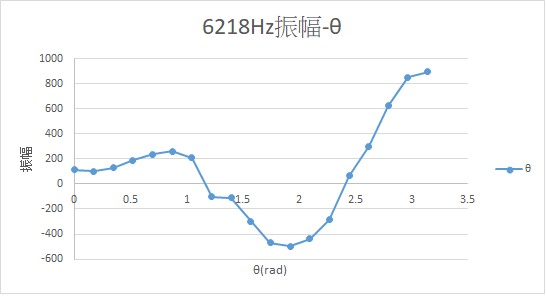
\includegraphics[width = .6\textwidth]{6218hz.png} \\
◆$7428 Hz$ \\
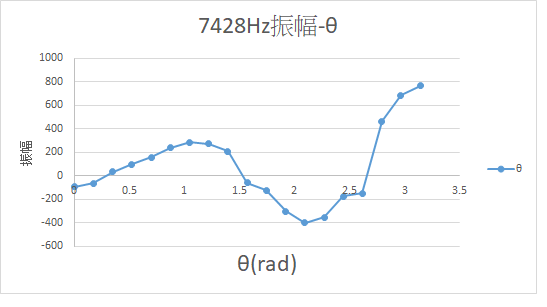
\includegraphics[width = .6\textwidth]{7428hz.png} \\

(3)各頻率($Hz$)之極座標掃描圖: \\
◆$2300 Hz$ \\
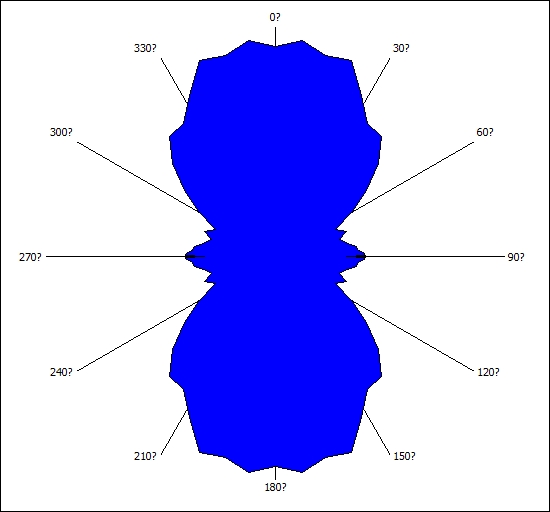
\includegraphics[width = .3\textwidth]{329_2300.jpg} \\
◆$3685.4 Hz$ \\
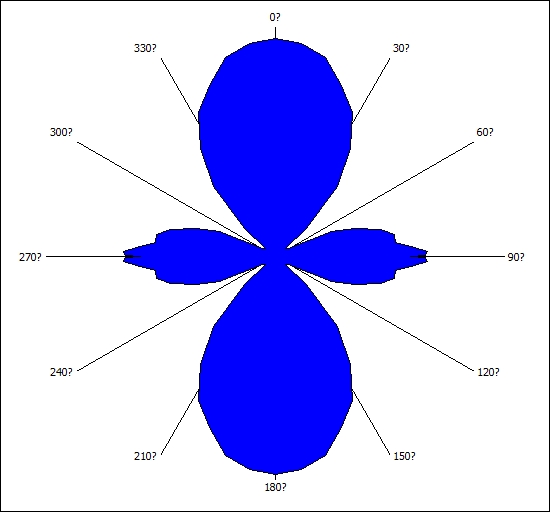
\includegraphics[width = .3\textwidth]{329_3685_4.jpg} \\
◆$4953 Hz$ \\
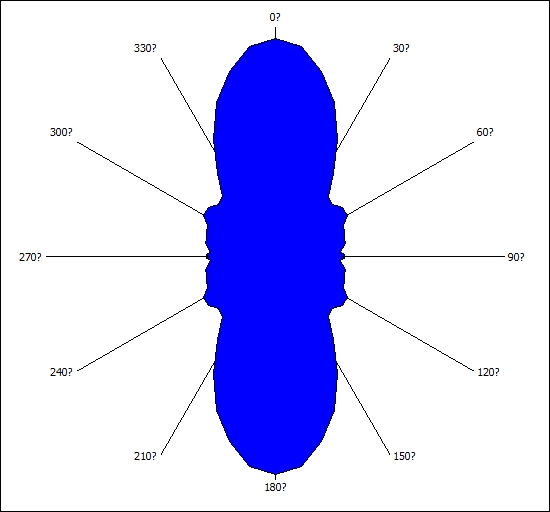
\includegraphics[width = .3\textwidth]{329_4953.jpg} \\
◆$4970 Hz$ \\
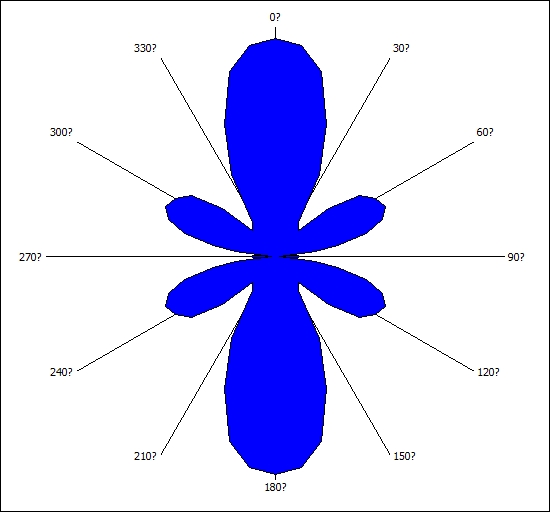
\includegraphics[width = .3\textwidth]{329_4970.jpg} \\
◆$6543 Hz$ \\
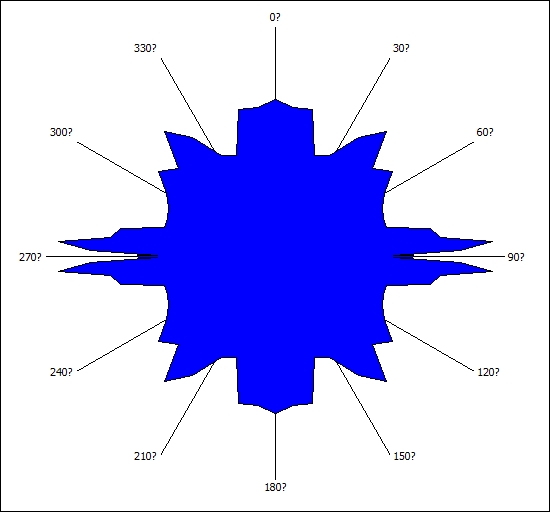
\includegraphics[width = .3\textwidth]{329_6543.jpg} \\
◆$7420 Hz$ \\
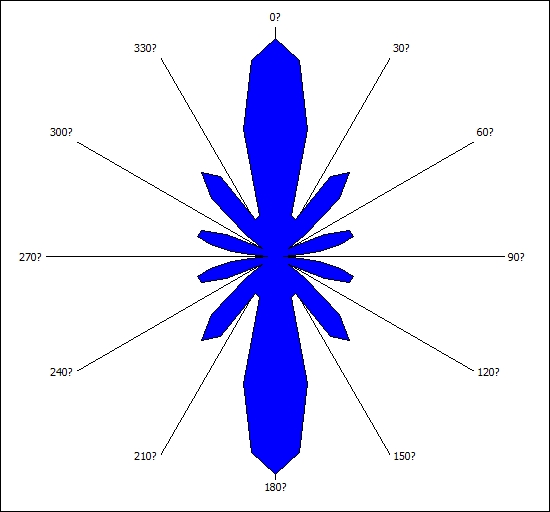
\includegraphics[width = .3\textwidth]{329_7420.jpg} \\
 \\
\newpage %強制分頁


% 資料分析數據整理
\begin{large}
\textbf{4.資料分析數據整理: } \\
\end{large}
(1)實驗裝置振幅($mV$)-頻率($Hz$) 關係圖 :\\ 
從圖中可得知,在2000$Hz$~8000$Hz$的頻域中,有5個明顯的peak,分別大約是在2300$Hz$、3690$Hz$、4975$Hz$、6218$Hz$與7428$Hz$。 \\
\\
(3)各頻率($Hz$)之極座標掃描圖: \\
上面各圖對照(3)之結果以及e3實驗講義中的$Fig. 1.4$ 可知以下對應: \\
◆$2300 Hz  \iff  Y^{0}_{1}(\theta,\varphi)$  \\
◆$3685.4 Hz  \iff  Y^{0}_{2}(\theta,\varphi)$  \\
◆$4970 Hz  \iff  Y^{0}_{3}(\theta,\varphi)$  \\
◆$6543 Hz  \iff  Y^{0}_{4}(\theta,\varphi)$  \\
◆$7420 Hz  \iff  Y^{0}_{5}(\theta,\varphi)$  \\
\\
(2)各頻率($Hz$)之振幅($mV$)-弧度($rad$) 關係圖: \\
從上面各圖對照(3)之結果以及e3實驗講義中的$Legendre Polynomiaals$圖型(如下圖)可相互對應: \\
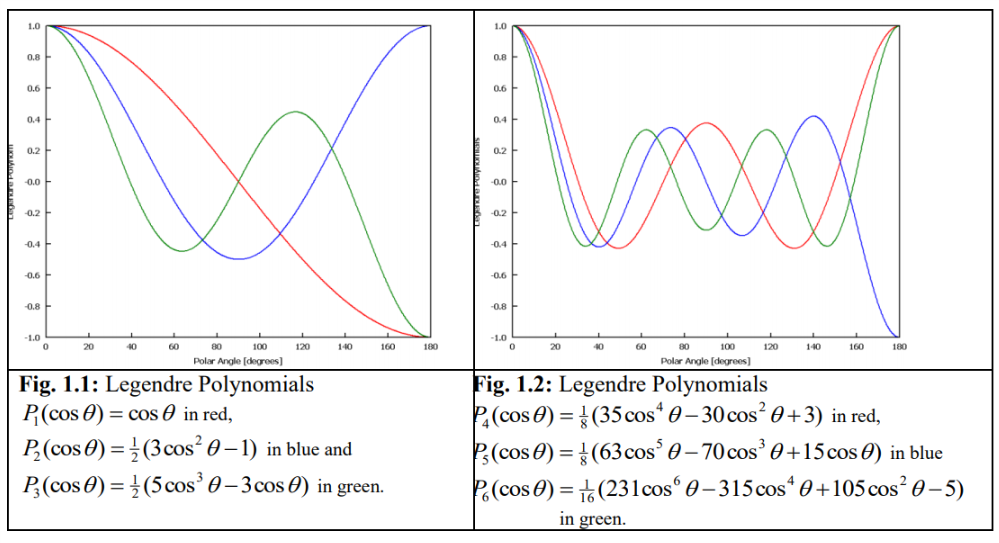
\includegraphics[width = .8\textwidth]{lp.png} \\
會發現,除了$2300 Hz$($Y^{0}_{1}(\theta,\varphi)$)、$3685.4 Hz$($Y^{0}_{2}(\theta,\varphi)$)之曲線趨勢近似之外,其餘4975$Hz$、6218$Hz$與7428$Hz$之波型並未如同$Y^{0}_{3}(\theta,\varphi)$、$Y^{0}_{4}(\theta,\varphi)$、$Y^{0}_{5}(\theta,\varphi)$有相近的曲折起伏,研判是手動實驗時取頻率之間隔太大以及多項人為操作誤差所致。 \\
\\

%%%%%%%%%%%%%%%%%%%%%%%%%%%%%%%%%%%%%%%

%%%%%%%%%%%%%%1~2頁%%%%%%%%%%%%%%%%%%

% 分析結果,系統誤差來源,數據或方式上的討論 等等,結論 (含問題回答或思考)
\begin{large}
\textbf{5.分析結果與誤差來源討論 :} \\
\end{large}
(1) 手動觀測之誤差來源可能為手掌於實驗過程中一直接觸Atom Analog金屬雙半球裝置上,手溫使鋁球內部聲音共振並非那麼完美理想。 \\
(2) 關於極座標做$Y^{0}_{x}(\theta,\varphi)$作圖之誤差可能是在選取欲掃描頻率時不夠準確(即選中並非振幅最大值)所致。\\

% 如何改進(可有可無,若有請討論原因)
\begin{large}
\textbf{6.如何改進實驗: } \\
\end{large}
(1) 在Atom Analog金屬雙半球裝置上之 $180^{\circ}$ 刻度刻痕可用黑色簽字筆加以強調使其更加醒目、使實驗對準角度時不用為了找尋刻度痕而花費過多時間。  \\
(2) 在音效卡自動掃頻實驗中可於實驗桌旁放置一平穩桌子來作為Atom Analog金屬雙半球裝置之實驗台,以避免電腦主機運作時震動所帶來的掃頻誤差。  \\

%列出猜考資料,各成員對此結報貢獻在何處
\begin{large}
\textbf{7.Reference: } \\
\end{large}
(1) e3上之實驗講義, "Quantum Analogs Modeling a Hydrogen Atom with a Spherical Resonator", 2018 \\
(2) Wikipedia, "Spherical harmonics",  https://en.wikipedia.org/wiki/Spherical Harmonics \\


\begin{large}
\textbf{8.組員貢獻分布: } \\
\end{large}
所有實驗與結報數據分析討論均是我們同組2人共同完成。 \\
(此次結報之~\LaTeX{} 格式繕打為 0412107 陳麒升負責 )

%$\sum_{i=1}^{n} f(x)$

\end{CJK*}
\end{document}